\documentclass[accentcolor=tud1b,colorbacktitle,landscape,german,presentation]{tudbeamer}

%Includes
\usepackage{float}
\usepackage{listings}
\usepackage{color}
\usepackage{graphicx}
\usepackage{epstopdf}
\usepackage{wrapfig}
\usepackage{pgfplots}
%Deutsche Silbentrennung
\usepackage[ngerman]{babel}
%Deutsche Umlaute
\usepackage[utf8]{inputenc}
\usepackage{adjustbox}
\usepackage{hyperref, tikz}
\usepackage{pdfpcnotes}

\setbeamerfont{note page}{size=\large}

\usetikzlibrary{shapes.misc, positioning, scopes}

\DeclareGraphicsExtensions{.pdf,.png,.jpg,.svg}
\graphicspath{ {./img/} }

\title[]{Entwicklung eines zentralen \\Steuerungsprogramms für einen \\Forschungsflugsimulator}
\subtitle{{\scriptsize Vortragender: Frederik Bark, Heiko Carrasco
	\\Team: Frederik Bark, Heiko Carrasco, Jonas Meurer und Leonardo Zaninelli}}
\institute{BP WS 2017/18 | Entwicklung eines zentralen Steuerungsprogramms für einen Forschungsflugsimulator}
\date{\today}

\newcommand{\ftitle}{
	\frametitle{\insertsectionhead \\ {\small \insertsubsectionhead}}
}
\begin{document}
%Deckblatt
\begin{titleframe}
	\begin{figure}
		\centering
		\includegraphics[scale=0.21]{simulator_3_intro}
	\end{figure}
	\pnote{Willkommen}
	\pnote{Gruppe 19}
\end{titleframe}


\section{Der Simulator}
\subsection{Aktuelle Situation}
\begin{frame}
	\ftitle
	\begin{figure}
		\centering
		\includegraphics[scale=0.055]{simulator_4}
	\end{figure}

	\pnote{Auftraggeber Institut für Flugsysteme und Regelungstechnik}
	\pnote{an der Lichtwiese}
	\pnote{wird zum Forschen im Bereich Führungsysteme (Flugverkehr) verwendet}
\end{frame}


\subsection{Aufbau des Systems}
\begin{frame}
	\ftitle
	\centering
	\begin{tikzpicture}[remember picture,overlay]
	\node[inner sep=0] at (current page.center)
	{		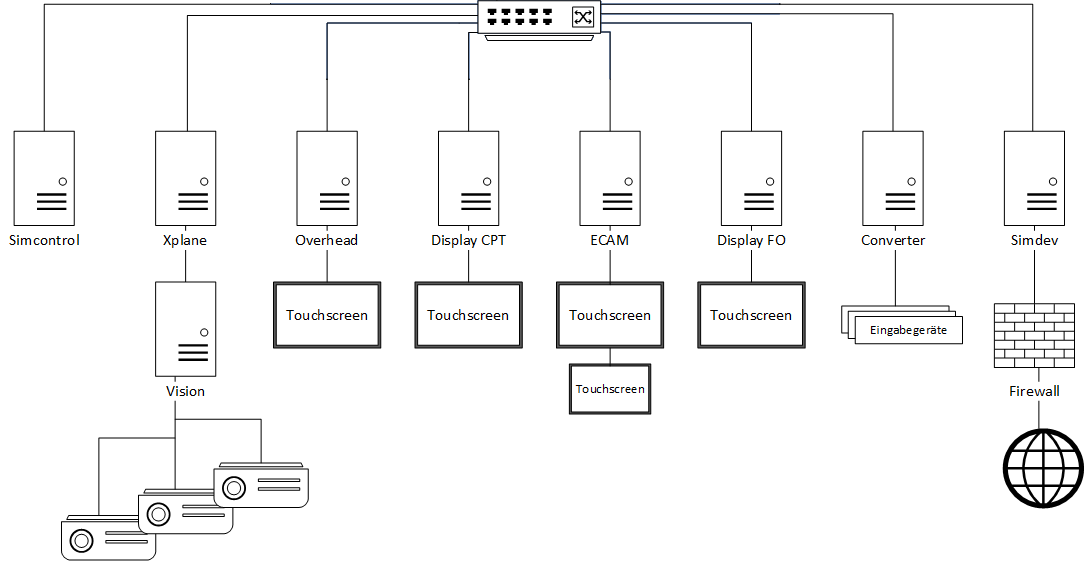
\includegraphics[scale=0.23]{aufbau_gesamt}};
	 \node (round) [line width=0.8pt,color=red, draw, rounded rectangle, yshift=-0.9cm, minimum height=1.3cm, minimum width=10cm] {};
		\node [color=red, below right= of round, yshift=0.9cm, xshift=-0.6cm] {Rechner};
	\end{tikzpicture}

\end{frame}


\begin{frame}
	\ftitle
	\centering
	\begin{tikzpicture}[remember picture,overlay]
	\node[inner sep=0] at (current page.center)
	{		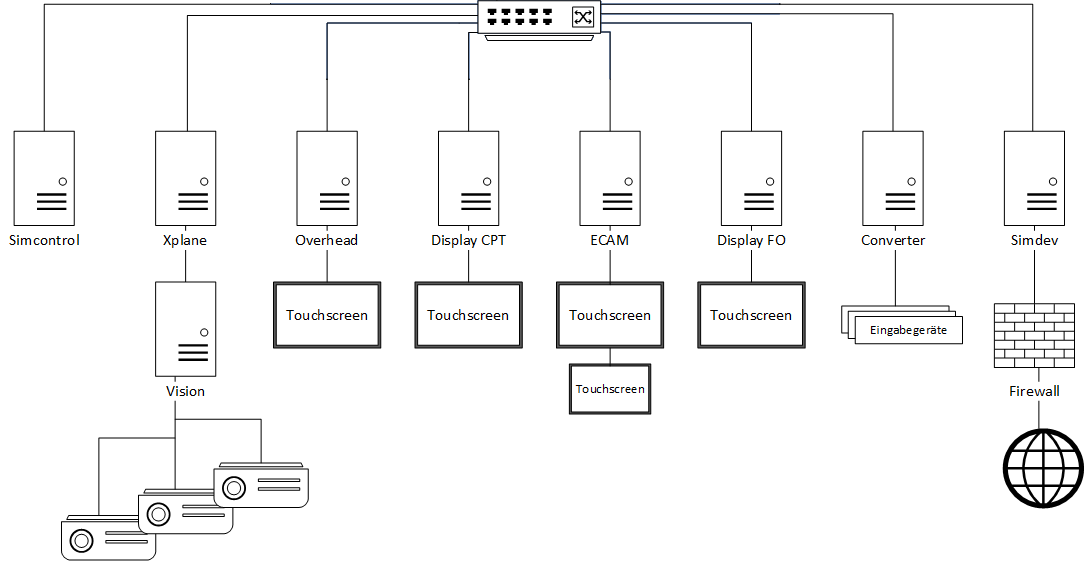
\includegraphics[scale=0.23]{aufbau_gesamt}};
	 \node (round) [line width=0.8pt,color=blue, draw, rounded rectangle, yshift=-2.2cm, minimum height=1.3cm, minimum width=10cm] {};
		\node [color=blue, below = of round, yshift=0.9cm, xshift=-0.0cm] {Ein- und Ausgabe};
	\end{tikzpicture}

\end{frame}

\subsection{Bisheriger Zustand}
\begin{frame}
	\ftitle
	\begin{itemize}
		\item Jeder Rechner muss per Hand gestartet werden\pause
		\item Programme müssen einzeln gestartet werden\pause
			\begin{itemize}
				\item Nicht immer wird alles benötigt/darf gestartet werden\pause
				\item Viel Wechsel zwischen den Rechnern nötig\pause
			\end{itemize}
	\end{itemize}
	\centering
	\vspace{0.5cm}
	\tikz[]\node[draw,minimum width=10cm,minimum height=3cm] {Bild vom KVM Switch};
\end{frame}

\section{Software}
\subsection{Gewünschte Features}
\begin{frame}
	\ftitle
	Features:
	\begin{itemize}
		\item Steuern von Rechnern und Programmen über eine Oberfläche\pause
		\item Erstellen von Ablaufplänen zum automatischen Start\pause
			\begin{itemize}
				\item Szenarien (Flugplatz, Flugzeug, \dots) wählbar machen\pause
				\item Plugins laden oder deaktivieren
			\end{itemize}
	\end{itemize}
\end{frame}

\subsection{Anforderungen}
\begin{frame}
	\ftitle
	\begin{itemize}
		\item Muss auf vielen unterschiedlichen Betriebssystem laufen\pause
		\item Einfache Bedienung für Mitarbeiter*innen\pause
		\item Muss weiterentwickelbar sein
	\end{itemize}
\end{frame}

\subsection{Lösung}
\begin{frame}
	\ftitle
	\begin{figure}
		\begin{overlayarea}{\textwidth}{4cm}
		\centering
		\only<1>{
\includegraphics[scale=0.42]{1}}
		\only<2>{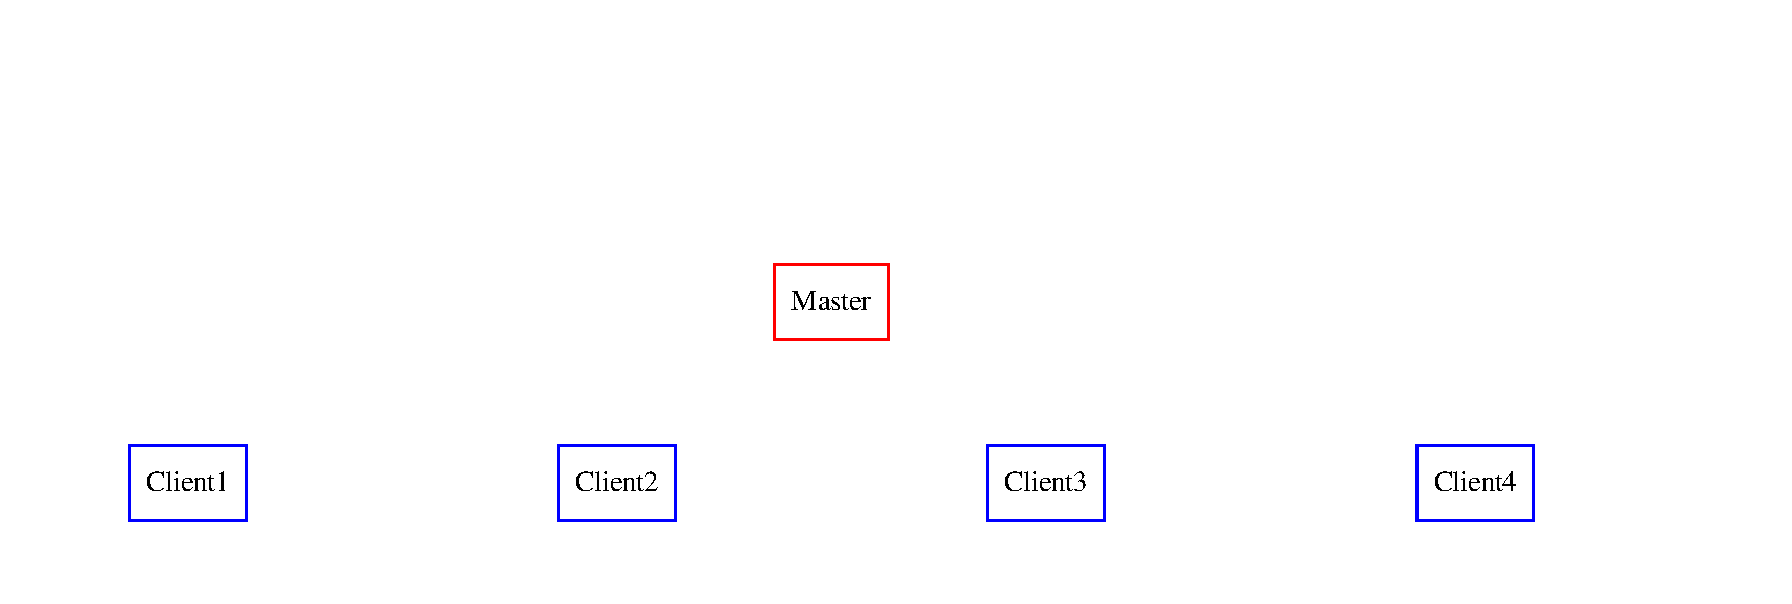
\includegraphics[scale=0.42]{2}}
		\only<3>{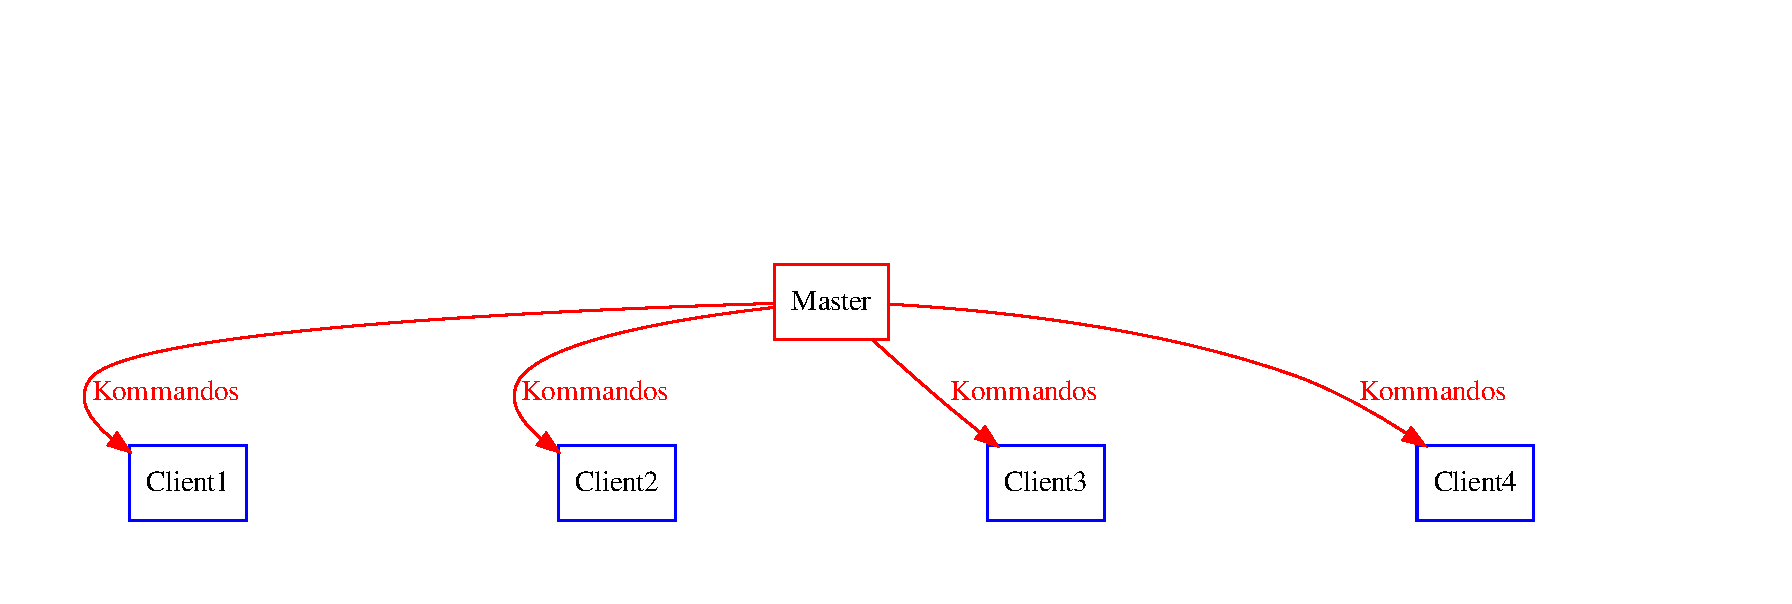
\includegraphics[scale=0.42]{3}}
		\only<4>{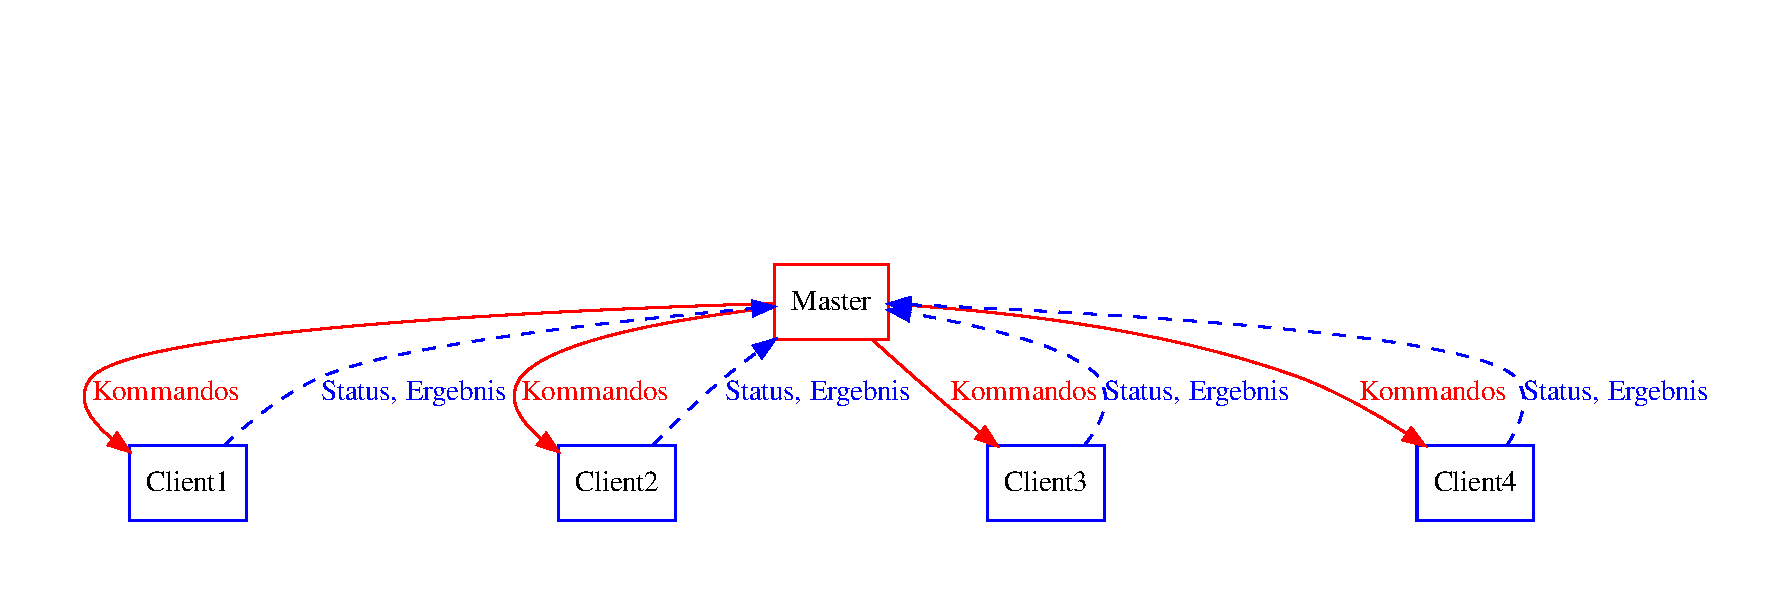
\includegraphics[scale=0.42]{4}}
		\only<5>{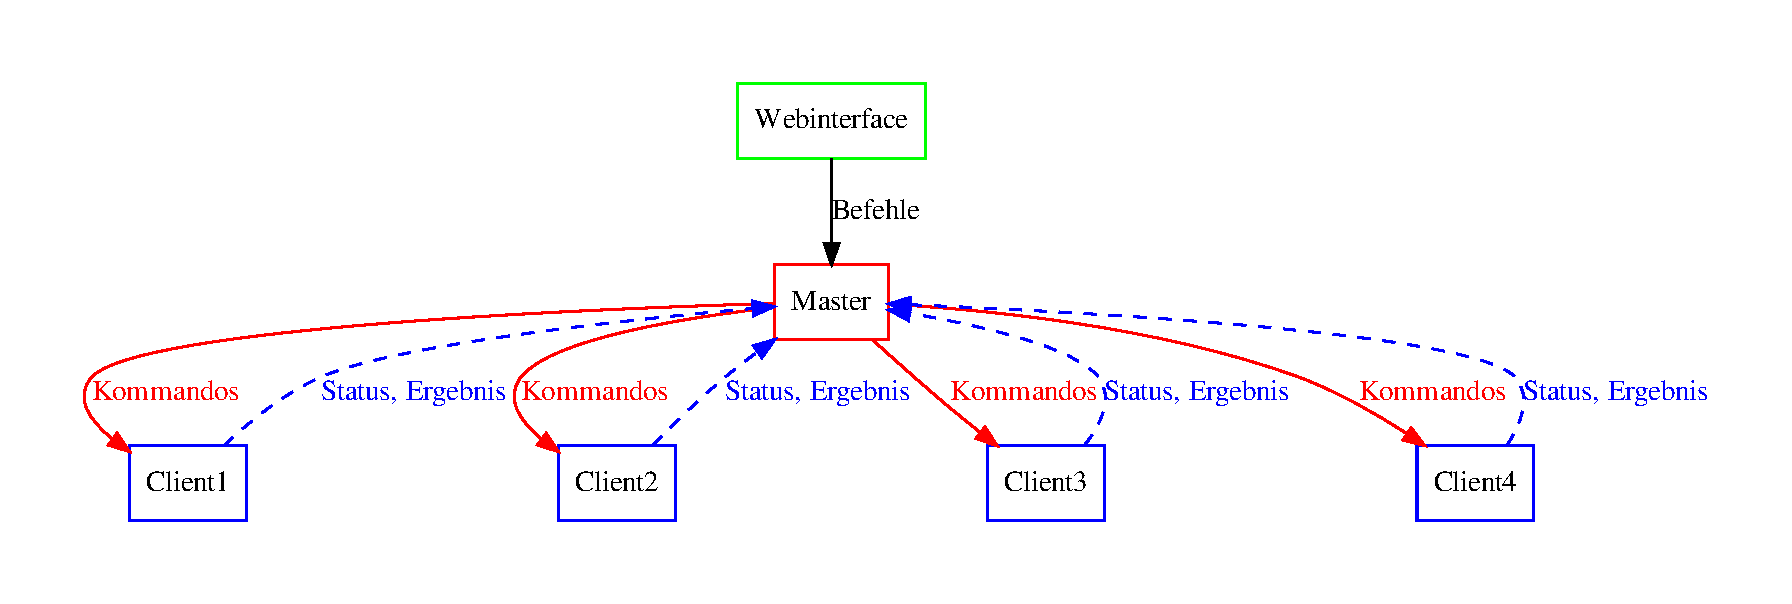
\includegraphics[scale=0.42]{6}}
		\end{overlayarea}
	\end{figure}
\end{frame}


\subsection{Fortschritt}
\begin{frame}
	\ftitle
	\vspace{-0.8cm}
	\begin{figure}
		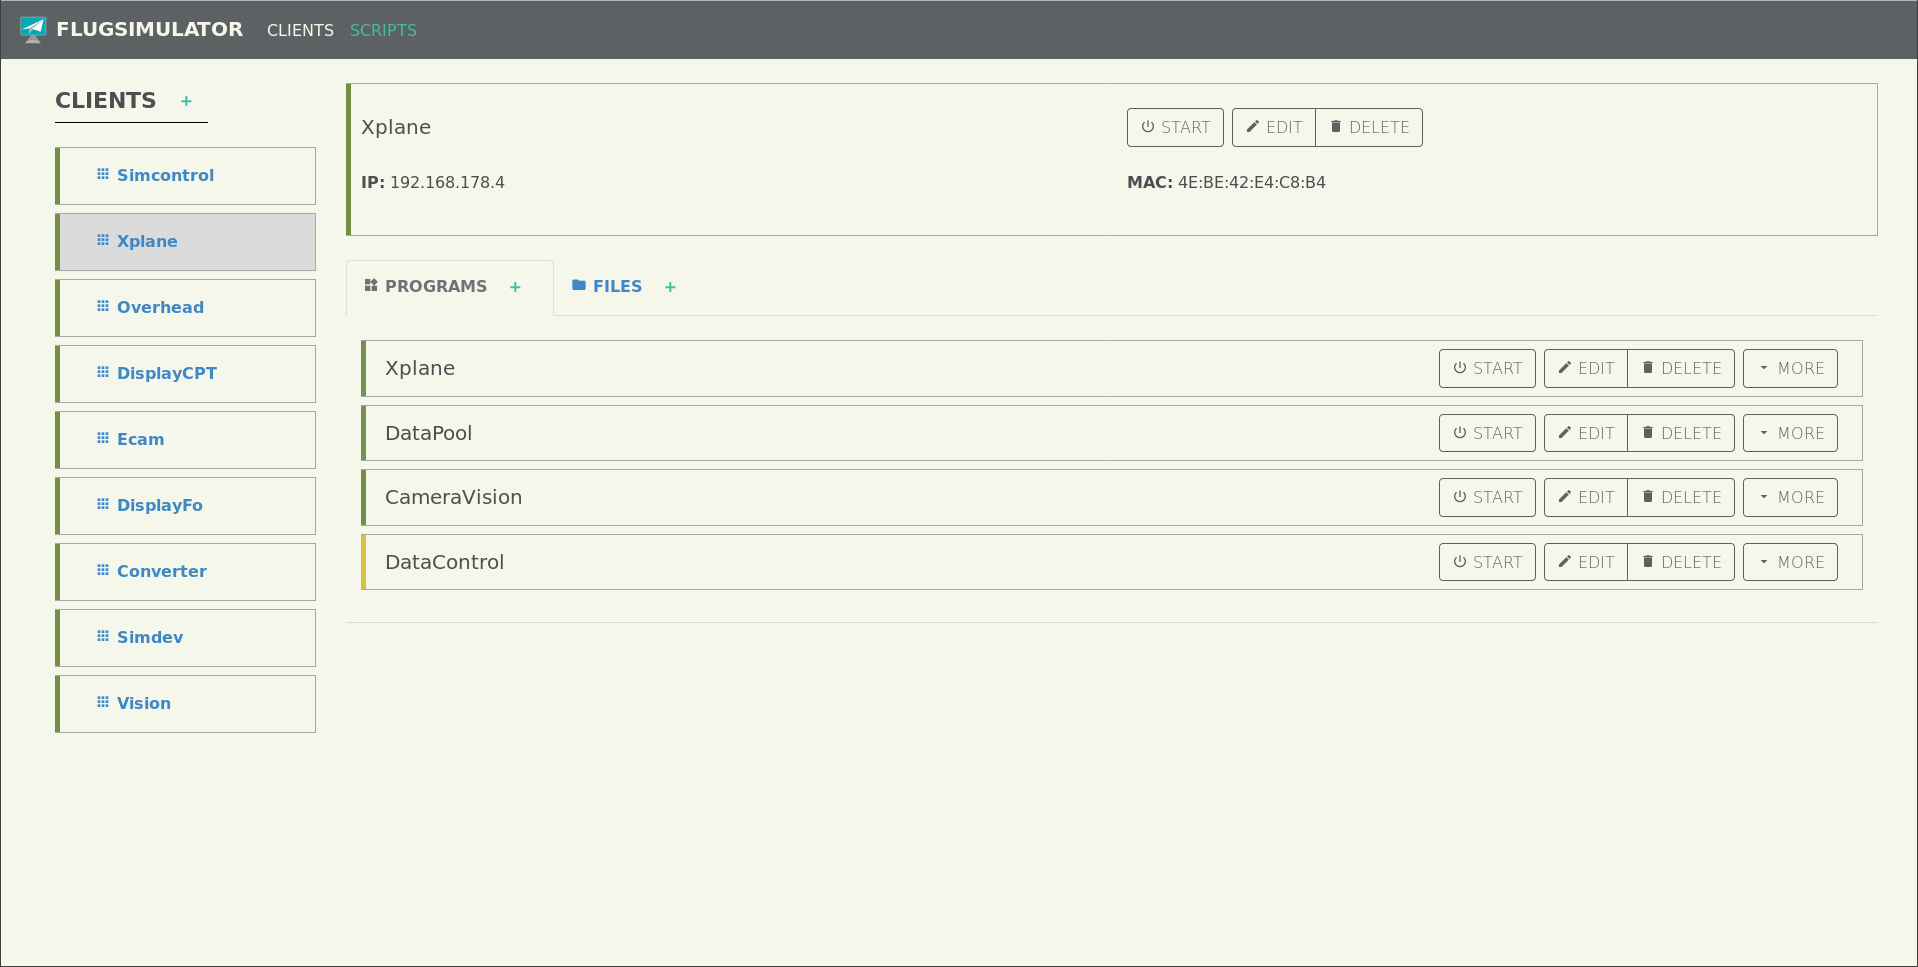
\includegraphics[scale=0.24]{interface}
	\end{figure}

	\pnote{hinzufügen von Clients im Webinterface}
	\pnote{hinzufügen von Programmen auf Clients im Webinterface}
	\pnote{wake on Lan}
	\pnote{grobe Implementierung von Master/Slave system}
\end{frame}

\section{Qualitätssicherung}
\subsection{Gesetzte Ziele}
\begin{frame}
	\ftitle
	\begin{itemize}
		\item Muss auf vielen unterschiedlichen Betriebssystem laufen
			\begin{itemize}
				\item <2->\textbf{Portabilität}
			\end{itemize}
		\item Einfache Bedienung für Mitarbeiter*innen
			\begin{itemize}
				\item <3->\textbf{Bedienbarkeit}
			\end{itemize}
		\item Muss weiterentwickelbar sein
			\begin{itemize}
				\item <4->\textbf{Korrektheit}
			\end{itemize}
	\end{itemize}

\end{frame}

\section{QS-Prozess}
\subsection{1. Automatisierte Tests}
\begin{frame}
	\ftitle
	\centering
	\vspace{-1.2cm}
	\begin{tikzpicture}
\node[inner sep=0pt] (marker) at (-4.45,2.3)
    {
\includegraphics[scale=0.06]{marker}};
\node[inner sep=0pt] (timeline) at (0,0)
    {\includegraphics[width=.8\textwidth]{qs-process}};
\end{tikzpicture}\pause
	\vspace{-4.5cm}
	\begin{itemize}
		\item QS-Ziele: \textbf{Portabilität, Korrekheit}\pause
	\end{itemize}
	\vspace{0.2cm}
	
\includegraphics[scale=0.2]{travisci}
	\hspace{0.1cm}
	
\includegraphics[scale=0.2]{appveyor}
	
\includegraphics[scale=0.18]{jenkins}
\end{frame}

\subsection{2. Coverage und Stilüberprüfung}
\begin{frame}
	\ftitle
	\centering
	\vspace{-1.2cm}
	\begin{tikzpicture}
\node[inner sep=0pt] (marker) at (-2.5,2.3)
    {
\includegraphics[scale=0.06]{marker}};
\node[inner sep=0pt] (timeline) at (0,0)
    {\includegraphics[width=.8\textwidth]{qs-process}};
\end{tikzpicture}\pause
	\vspace{-4.5cm}
	\begin{itemize}
		\item QS-Ziel: \textbf{Korrektheit}\pause
	\end{itemize}
	\vspace{0.2cm}
	
\includegraphics[scale=0.2]{coveralls}
	\hspace{0.1cm}
	
\includegraphics[scale=0.14]{codacy}
\end{frame}


\begin{frame}
	\ftitle
	\vspace{-0.5cm}
	\begin{figure}
		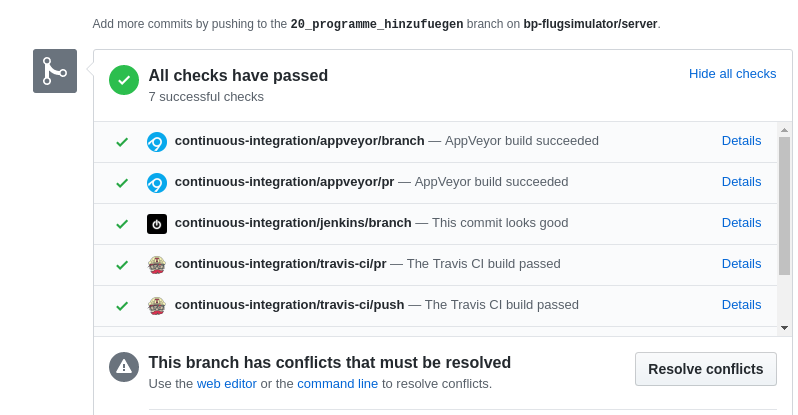
\includegraphics[scale=0.4]{github_integration}
	\end{figure}

	\pnote{für jede Userstory wird ein Pullrequests auf Github gemacht}
	\pnote{dient auch als Forum für Implementierungen}
\end{frame}

\subsection{3. Review durch anderen Entwickler}
\begin{frame}
	\ftitle
	\centering
	\vspace{-1.2cm}
	\begin{tikzpicture}
\node[inner sep=0pt] (marker) at (-0.55,2.3)
    {
\includegraphics[scale=0.06]{marker}};
\node[inner sep=0pt] (timeline) at (0,0)
    {\includegraphics[width=.8\textwidth]{qs-process}};
\end{tikzpicture}
	\vspace{-4.5cm}
	\begin{itemize}
		\item Review wird von einem anderen Entwickler durchgeführt\pause
		\item Checkliste mit Punkten wie z.B. Dokumentation
	\end{itemize}
\end{frame}

\begin{frame}
	\ftitle
	\begin{figure}
		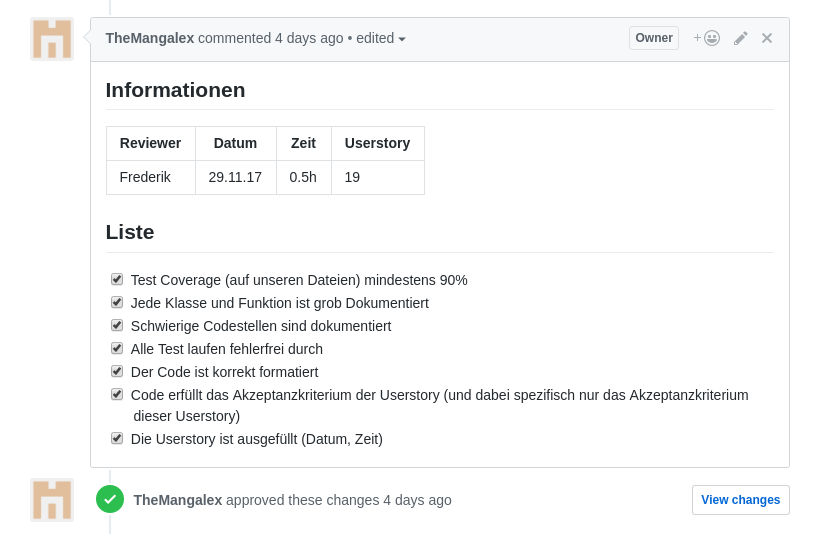
\includegraphics[scale=0.29]{github_list}
	\end{figure}
	\pnote{falls eine Punkt nicht erfüllt wird, muss der Entwickler der Userstory
		das Problem beheben}
\end{frame}

\subsection{4. Nutzerstudie am Fachgebiet}
\begin{frame}
	\ftitle
	\centering
	\vspace{-1.2cm}
	\begin{tikzpicture}
\node[inner sep=0pt] (marker) at (1.42,2.3)
    {
\includegraphics[scale=0.06]{marker}};
\node[inner sep=0pt] (timeline) at (0,0)
    {\includegraphics[width=.8\textwidth]{qs-process}};
\end{tikzpicture}
	\vspace{-4.5cm}
	\begin{itemize}
		\item Nutzerstudie zum Test der Bedienbarkeit\pause
		\item Durchführung Anfang 2018\pause
		\item QS-Ziel: \textbf{Bedienbarkeit}
	\end{itemize}
\end{frame}


\subsection{5. Abnahme durch die Auftraggeber}
\begin{frame}
	\ftitle
	\centering
	\vspace{-1.2cm}
	\begin{tikzpicture}
\node[inner sep=0pt] (marker) at (3.39,2.3)
    {
\includegraphics[scale=0.06]{marker}};
\node[inner sep=0pt] (timeline) at (0,0)
    {\includegraphics[width=.8\textwidth]{qs-process}};
\end{tikzpicture}
	\vspace{-4.5cm}
	\begin{itemize}
		\item Auftraggeber erhalten Zusammenfassung\pause
		\item Anmerkungen für die nächste Iteration
	\end{itemize}
\end{frame}


\end{document}
